\documentclass[twoside]{book}

% Packages required by doxygen
\usepackage{fixltx2e}
\usepackage{calc}
\usepackage{doxygen}
\usepackage[export]{adjustbox} % also loads graphicx
\usepackage{graphicx}
\usepackage[utf8]{inputenc}
\usepackage{makeidx}
\usepackage{multicol}
\usepackage{multirow}
\PassOptionsToPackage{warn}{textcomp}
\usepackage{textcomp}
\usepackage[nointegrals]{wasysym}
\usepackage[table]{xcolor}

% Font selection
\usepackage[T1]{fontenc}
\usepackage[scaled=.90]{helvet}
\usepackage{courier}
\usepackage{amssymb}
\usepackage{sectsty}
\renewcommand{\familydefault}{\sfdefault}
\allsectionsfont{%
  \fontseries{bc}\selectfont%
  \color{darkgray}%
}
\renewcommand{\DoxyLabelFont}{%
  \fontseries{bc}\selectfont%
  \color{darkgray}%
}
\newcommand{\+}{\discretionary{\mbox{\scriptsize$\hookleftarrow$}}{}{}}

% Page & text layout
\usepackage{geometry}
\geometry{%
  a4paper,%
  top=2.5cm,%
  bottom=2.5cm,%
  left=2.5cm,%
  right=2.5cm%
}
\tolerance=750
\hfuzz=15pt
\hbadness=750
\setlength{\emergencystretch}{15pt}
\setlength{\parindent}{0cm}
\setlength{\parskip}{3ex plus 2ex minus 2ex}
\makeatletter
\renewcommand{\paragraph}{%
  \@startsection{paragraph}{4}{0ex}{-1.0ex}{1.0ex}{%
    \normalfont\normalsize\bfseries\SS@parafont%
  }%
}
\renewcommand{\subparagraph}{%
  \@startsection{subparagraph}{5}{0ex}{-1.0ex}{1.0ex}{%
    \normalfont\normalsize\bfseries\SS@subparafont%
  }%
}
\makeatother

% Headers & footers
\usepackage{fancyhdr}
\pagestyle{fancyplain}
\fancyhead[LE]{\fancyplain{}{\bfseries\thepage}}
\fancyhead[CE]{\fancyplain{}{}}
\fancyhead[RE]{\fancyplain{}{\bfseries\leftmark}}
\fancyhead[LO]{\fancyplain{}{\bfseries\rightmark}}
\fancyhead[CO]{\fancyplain{}{}}
\fancyhead[RO]{\fancyplain{}{\bfseries\thepage}}
\fancyfoot[LE]{\fancyplain{}{}}
\fancyfoot[CE]{\fancyplain{}{}}
\fancyfoot[RE]{\fancyplain{}{\bfseries\scriptsize Generated by Doxygen }}
\fancyfoot[LO]{\fancyplain{}{\bfseries\scriptsize Generated by Doxygen }}
\fancyfoot[CO]{\fancyplain{}{}}
\fancyfoot[RO]{\fancyplain{}{}}
\renewcommand{\footrulewidth}{0.4pt}
\renewcommand{\chaptermark}[1]{%
  \markboth{#1}{}%
}
\renewcommand{\sectionmark}[1]{%
  \markright{\thesection\ #1}%
}

% Indices & bibliography
\usepackage{natbib}
\usepackage[titles]{tocloft}
\setcounter{tocdepth}{3}
\setcounter{secnumdepth}{5}
\makeindex

% Custom commands
\newcommand{\clearemptydoublepage}{%
  \newpage{\pagestyle{empty}\cleardoublepage}%
}

\usepackage{caption}
\captionsetup{labelsep=space,justification=centering,font={bf},singlelinecheck=off,skip=4pt,position=top}

%===== C O N T E N T S =====

\begin{document}

% Titlepage & ToC
\pagenumbering{alph}
\begin{titlepage}
\vspace*{7cm}
\begin{center}%
{\Large 2gether -\/ Reliability Assessment Model (R\+AM) \\[1ex]\large v1.\+0 }\\
\vspace*{1cm}
{\large Generated by Doxygen 1.8.14}\\
\end{center}
\end{titlepage}
\clearemptydoublepage
\pagenumbering{roman}
\tableofcontents
\clearemptydoublepage
\pagenumbering{arabic}

%--- Begin generated contents ---
\chapter{Namespace Index}
\section{Namespace List}
Here is a list of all namespaces with brief descriptions\+:\begin{DoxyCompactList}
\item\contentsline{section}{\textbf{ gnfnc} }{\pageref{namespacegnfnc}}{}
\end{DoxyCompactList}

\chapter{Class Index}
\section{Class List}
Here are the classes, structs, unions and interfaces with brief descriptions\+:\begin{DoxyCompactList}
\item\contentsline{section}{\textbf{ Artist} }{\pageref{class_artist}}{}
\item\contentsline{section}{\textbf{ Artwork} }{\pageref{class_artwork}}{}
\item\contentsline{section}{\textbf{ Rating} }{\pageref{class_rating}}{}
\end{DoxyCompactList}

\chapter{File Index}
\section{File List}
Here is a list of all files with brief descriptions\+:\begin{DoxyCompactList}
\item\contentsline{section}{\textbf{ Artist.\+cpp} }{\pageref{_artist_8cpp}}{}
\item\contentsline{section}{\textbf{ Artist.\+h} }{\pageref{_artist_8h}}{}
\item\contentsline{section}{\textbf{ Artwork.\+cpp} }{\pageref{_artwork_8cpp}}{}
\item\contentsline{section}{\textbf{ Artwork.\+h} }{\pageref{_artwork_8h}}{}
\item\contentsline{section}{\textbf{ dirent.\+h} }{\pageref{dirent_8h}}{}
\item\contentsline{section}{\textbf{ Generic\+Func.\+cpp} }{\pageref{_generic_func_8cpp}}{}
\item\contentsline{section}{\textbf{ Generic\+Func.\+h} }{\pageref{_generic_func_8h}}{}
\item\contentsline{section}{\textbf{ main.\+cpp} }{\pageref{main_8cpp}}{}
\item\contentsline{section}{\textbf{ Rating.\+cpp} }{\pageref{_rating_8cpp}}{}
\item\contentsline{section}{\textbf{ Rating.\+h} }{\pageref{_rating_8h}}{}
\end{DoxyCompactList}

\chapter{Namespace Documentation}
\section{gnfnc Namespace Reference}
\label{namespacegnfnc}\index{gnfnc@{gnfnc}}
\subsection*{Functions}
\begin{DoxyCompactItemize}
\item 
std\+::string \textbf{ get\+Executable\+Path} ()
\item 
std\+::string \textbf{ get\+Executable\+Path\+And\+Match\+It\+With\+Filename} (const std\+::string \&file\+Name)
\end{DoxyCompactItemize}


\subsection{Function Documentation}
\mbox{\label{namespacegnfnc_a83d25b352dc66d2317f398c5a3c67f81}} 
\index{gnfnc@{gnfnc}!get\+Executable\+Path@{get\+Executable\+Path}}
\index{get\+Executable\+Path@{get\+Executable\+Path}!gnfnc@{gnfnc}}
\subsubsection{get\+Executable\+Path()}
{\footnotesize\ttfamily std\+::string gnfnc\+::get\+Executable\+Path (\begin{DoxyParamCaption}{ }\end{DoxyParamCaption})}

Returns the absolute path of the executable\textquotesingle{}s directory. \begin{DoxyReturn}{Returns}
the absolute path of the executable\textquotesingle{}s directory. 
\end{DoxyReturn}


Definition at line 8 of file Generic\+Func.\+cpp.

\mbox{\label{namespacegnfnc_adf0284ac1df7768c93180ada79054488}} 
\index{gnfnc@{gnfnc}!get\+Executable\+Path\+And\+Match\+It\+With\+Filename@{get\+Executable\+Path\+And\+Match\+It\+With\+Filename}}
\index{get\+Executable\+Path\+And\+Match\+It\+With\+Filename@{get\+Executable\+Path\+And\+Match\+It\+With\+Filename}!gnfnc@{gnfnc}}
\subsubsection{get\+Executable\+Path\+And\+Match\+It\+With\+Filename()}
{\footnotesize\ttfamily std\+::string gnfnc\+::get\+Executable\+Path\+And\+Match\+It\+With\+Filename (\begin{DoxyParamCaption}\item[{const std\+::string \&}]{file\+Name }\end{DoxyParamCaption})}

Returns the absolute path a file located in the executable\textquotesingle{}s directory. 
\begin{DoxyParams}{Parameters}
{\em file\+Name} & the name of the file (e.\+g., file.\+txt) \\
\hline
\end{DoxyParams}
\begin{DoxyReturn}{Returns}
the absolute path of the file 
\end{DoxyReturn}


Definition at line 17 of file Generic\+Func.\+cpp.


\chapter{Class Documentation}
\section{Artist Class Reference}
\label{class_artist}\index{Artist@{Artist}}


{\ttfamily \#include $<$Artist.\+h$>$}

\subsection*{Public Member Functions}
\begin{DoxyCompactItemize}
\item 
\textbf{ Artist} ()
\item 
\textbf{ Artist} (int id)
\item 
\textbf{ $\sim$\+Artist} ()
\item 
void \textbf{ set\+ID} (int id)
\item 
int \textbf{ get\+ID} () const
\item 
void \textbf{ add\+R\+A\+Mrep} (double R\+A\+Mrep)
\item 
void \textbf{ add\+B\+E\+Nrep} (double B\+E\+Nrep)
\item 
void \textbf{ save\+R\+A\+Mreps} ()
\item 
void \textbf{ save\+B\+E\+Nreps} ()
\item 
void \textbf{ set\+Malicious} (bool malicious)
\item 
bool \textbf{ is\+Malicious} () const
\item 
void \textbf{ add\+Rating} (\textbf{ Rating} $\ast$rating)
\item 
void \textbf{ compute\+Average\+Rating\+Received} ()
\item 
double \textbf{ get\+Average\+Rating\+Received} () const
\item 
void \textbf{ compute\+Average\+Rating\+Given} ()
\item 
double \textbf{ get\+Average\+Rating\+Given} () const
\item 
void \textbf{ add\+Artwork} (int artwork\+ID, \textbf{ Artwork} $\ast$artwork)
\item 
\textbf{ Artwork} $\ast$ \textbf{ get\+Artwork} (int artwork\+ID)
\item 
std\+::map$<$ int, \textbf{ Artwork} $\ast$ $>$ $\ast$ \textbf{ get\+Artworks} ()
\item 
int \textbf{ get\+Num\+Of\+Artworks} ()
\item 
bool \textbf{ artwork\+Exists} (int artwork\+ID)
\item 
void \textbf{ print\+Artworks\+I\+Ds} ()
\end{DoxyCompactItemize}


\subsection{Detailed Description}


Definition at line 9 of file Artist.\+h.



\subsection{Constructor \& Destructor Documentation}
\mbox{\label{class_artist_ad49ef7a2d2847076e737a2836e8915ab}} 
\index{Artist@{Artist}!Artist@{Artist}}
\index{Artist@{Artist}!Artist@{Artist}}
\subsubsection{Artist()\hspace{0.1cm}{\footnotesize\ttfamily [1/2]}}
{\footnotesize\ttfamily Artist\+::\+Artist (\begin{DoxyParamCaption}{ }\end{DoxyParamCaption})}

Default constructor. 

Definition at line 10 of file Artist.\+cpp.

\mbox{\label{class_artist_a486d55ca54ff3a9df584889466c7cc44}} 
\index{Artist@{Artist}!Artist@{Artist}}
\index{Artist@{Artist}!Artist@{Artist}}
\subsubsection{Artist()\hspace{0.1cm}{\footnotesize\ttfamily [2/2]}}
{\footnotesize\ttfamily Artist\+::\+Artist (\begin{DoxyParamCaption}\item[{int}]{id }\end{DoxyParamCaption})}

Constructor. 
\begin{DoxyParams}{Parameters}
{\em id} & the ID of the \doxyref{Artist}{p.}{class_artist} object. \\
\hline
\end{DoxyParams}


Definition at line 18 of file Artist.\+cpp.

\mbox{\label{class_artist_ab07f3ad7c2ebc2663e77a1663a705fe3}} 
\index{Artist@{Artist}!````~Artist@{$\sim$\+Artist}}
\index{````~Artist@{$\sim$\+Artist}!Artist@{Artist}}
\subsubsection{$\sim$\+Artist()}
{\footnotesize\ttfamily Artist\+::$\sim$\+Artist (\begin{DoxyParamCaption}{ }\end{DoxyParamCaption})}

Destructor. 

Definition at line 26 of file Artist.\+cpp.



\subsection{Member Function Documentation}
\mbox{\label{class_artist_ab540e33cd89be910d337f252805bc57d}} 
\index{Artist@{Artist}!add\+Artwork@{add\+Artwork}}
\index{add\+Artwork@{add\+Artwork}!Artist@{Artist}}
\subsubsection{add\+Artwork()}
{\footnotesize\ttfamily void Artist\+::add\+Artwork (\begin{DoxyParamCaption}\item[{int}]{artwork\+ID,  }\item[{\textbf{ Artwork} $\ast$}]{artwork }\end{DoxyParamCaption})}

Adds a new \doxyref{Artwork}{p.}{class_artwork} object in the list of \doxyref{Artwork}{p.}{class_artwork} objects of the artist. 
\begin{DoxyParams}{Parameters}
{\em artwork\+ID} & the ID of the \doxyref{Artwork}{p.}{class_artwork} object. \\
\hline
{\em artwork} & the \doxyref{Artwork}{p.}{class_artwork} object. \\
\hline
\end{DoxyParams}


Definition at line 153 of file Artist.\+cpp.

\mbox{\label{class_artist_a004975042019f53cefe0d8c94903d845}} 
\index{Artist@{Artist}!add\+B\+E\+Nrep@{add\+B\+E\+Nrep}}
\index{add\+B\+E\+Nrep@{add\+B\+E\+Nrep}!Artist@{Artist}}
\subsubsection{add\+B\+E\+Nrep()}
{\footnotesize\ttfamily void Artist\+::add\+B\+E\+Nrep (\begin{DoxyParamCaption}\item[{double}]{B\+E\+Nrep }\end{DoxyParamCaption})}

Adds a new benchmark reputation value in the vector of benchmark reputation values. 
\begin{DoxyParams}{Parameters}
{\em B\+E\+Nrep} & the benchmark reputation value to be added. \\
\hline
\end{DoxyParams}


Definition at line 64 of file Artist.\+cpp.

\mbox{\label{class_artist_a8e7f7f2c9aa71a5ab6c30363387d1462}} 
\index{Artist@{Artist}!add\+R\+A\+Mrep@{add\+R\+A\+Mrep}}
\index{add\+R\+A\+Mrep@{add\+R\+A\+Mrep}!Artist@{Artist}}
\subsubsection{add\+R\+A\+Mrep()}
{\footnotesize\ttfamily void Artist\+::add\+R\+A\+Mrep (\begin{DoxyParamCaption}\item[{double}]{R\+A\+Mrep }\end{DoxyParamCaption})}

Adds a new R\+AM reputation value in the vector of R\+AM reputation values. 
\begin{DoxyParams}{Parameters}
{\em R\+A\+Mrep} & the R\+AM reputation value to be added. \\
\hline
\end{DoxyParams}


Definition at line 59 of file Artist.\+cpp.

\mbox{\label{class_artist_ab829e8b608a24fac68f7b578c4414ca1}} 
\index{Artist@{Artist}!add\+Rating@{add\+Rating}}
\index{add\+Rating@{add\+Rating}!Artist@{Artist}}
\subsubsection{add\+Rating()}
{\footnotesize\ttfamily void Artist\+::add\+Rating (\begin{DoxyParamCaption}\item[{\textbf{ Rating} $\ast$}]{rating }\end{DoxyParamCaption})}

Adds a new \doxyref{Rating}{p.}{class_rating} object (i.\+e., pointer to \doxyref{Rating}{p.}{class_rating} object) to the vector of \doxyref{Rating}{p.}{class_rating} objects (i.\+e., vector of pointers to rating objects). 
\begin{DoxyParams}{Parameters}
{\em rating} & the new \doxyref{Rating}{p.}{class_rating} object. \\
\hline
\end{DoxyParams}


Definition at line 111 of file Artist.\+cpp.

\mbox{\label{class_artist_a7717c5307eb7c3a76695f114202ce1f0}} 
\index{Artist@{Artist}!artwork\+Exists@{artwork\+Exists}}
\index{artwork\+Exists@{artwork\+Exists}!Artist@{Artist}}
\subsubsection{artwork\+Exists()}
{\footnotesize\ttfamily bool Artist\+::artwork\+Exists (\begin{DoxyParamCaption}\item[{int}]{artwork\+ID }\end{DoxyParamCaption})}

Checks if an \doxyref{Artwork}{p.}{class_artwork} object with specific ID exists in the list of \doxyref{Artwork}{p.}{class_artwork} objects of the \doxyref{Artist}{p.}{class_artist}. 
\begin{DoxyParams}{Parameters}
{\em artwork\+ID} & the ID of the \doxyref{Artwork}{p.}{class_artwork} object. \\
\hline
\end{DoxyParams}
\begin{DoxyReturn}{Returns}
true if the \doxyref{Artwork}{p.}{class_artwork} object belongs to the \doxyref{Artist}{p.}{class_artist}, false otherwise. 
\end{DoxyReturn}


Definition at line 147 of file Artist.\+cpp.

\mbox{\label{class_artist_a7fe3ceeb3051139945f18445a420b3c8}} 
\index{Artist@{Artist}!compute\+Average\+Rating\+Given@{compute\+Average\+Rating\+Given}}
\index{compute\+Average\+Rating\+Given@{compute\+Average\+Rating\+Given}!Artist@{Artist}}
\subsubsection{compute\+Average\+Rating\+Given()}
{\footnotesize\ttfamily void Artist\+::compute\+Average\+Rating\+Given (\begin{DoxyParamCaption}{ }\end{DoxyParamCaption})}

Computes the average of all ratings given by the \doxyref{Artist}{p.}{class_artist} for the artworks of other artists. 

Definition at line 132 of file Artist.\+cpp.

\mbox{\label{class_artist_a1a5e102b899f7c61ffe4f4f7497ef800}} 
\index{Artist@{Artist}!compute\+Average\+Rating\+Received@{compute\+Average\+Rating\+Received}}
\index{compute\+Average\+Rating\+Received@{compute\+Average\+Rating\+Received}!Artist@{Artist}}
\subsubsection{compute\+Average\+Rating\+Received()}
{\footnotesize\ttfamily void Artist\+::compute\+Average\+Rating\+Received (\begin{DoxyParamCaption}{ }\end{DoxyParamCaption})}

Computes the average of the ratings received for all the artworks of the \doxyref{Artist}{p.}{class_artist}. 

Definition at line 116 of file Artist.\+cpp.

\mbox{\label{class_artist_aa42eb1e5cc2672faebf54d84da83d0f3}} 
\index{Artist@{Artist}!get\+Artwork@{get\+Artwork}}
\index{get\+Artwork@{get\+Artwork}!Artist@{Artist}}
\subsubsection{get\+Artwork()}
{\footnotesize\ttfamily \textbf{ Artwork} $\ast$ Artist\+::get\+Artwork (\begin{DoxyParamCaption}\item[{int}]{artwork\+ID }\end{DoxyParamCaption})}

Returns an \doxyref{Artwork}{p.}{class_artwork} object from the list of \doxyref{Artwork}{p.}{class_artwork} objects of the \doxyref{Artist}{p.}{class_artist}. 
\begin{DoxyParams}{Parameters}
{\em artwork\+ID} & the ID of the \doxyref{Artwork}{p.}{class_artwork} object. \\
\hline
\end{DoxyParams}
\begin{DoxyReturn}{Returns}
the \doxyref{Artwork}{p.}{class_artwork} object. 
\end{DoxyReturn}


Definition at line 161 of file Artist.\+cpp.

\mbox{\label{class_artist_acdfcaf619563c7aec743887d19e5e2b1}} 
\index{Artist@{Artist}!get\+Artworks@{get\+Artworks}}
\index{get\+Artworks@{get\+Artworks}!Artist@{Artist}}
\subsubsection{get\+Artworks()}
{\footnotesize\ttfamily std\+::map$<$ int, \textbf{ Artwork} $\ast$ $>$ $\ast$ Artist\+::get\+Artworks (\begin{DoxyParamCaption}{ }\end{DoxyParamCaption})}

Returns the list of \doxyref{Artwork}{p.}{class_artwork} objects of the \doxyref{Artist}{p.}{class_artist}. \begin{DoxyReturn}{Returns}
the list of \doxyref{Artwork}{p.}{class_artwork} objects of the \doxyref{Artist}{p.}{class_artist}. 
\end{DoxyReturn}


Definition at line 182 of file Artist.\+cpp.

\mbox{\label{class_artist_a4719d8f710f647ff68aadcfa35667b3b}} 
\index{Artist@{Artist}!get\+Average\+Rating\+Given@{get\+Average\+Rating\+Given}}
\index{get\+Average\+Rating\+Given@{get\+Average\+Rating\+Given}!Artist@{Artist}}
\subsubsection{get\+Average\+Rating\+Given()}
{\footnotesize\ttfamily double Artist\+::get\+Average\+Rating\+Given (\begin{DoxyParamCaption}{ }\end{DoxyParamCaption}) const}

Returns the average of all ratings given by the \doxyref{Artist}{p.}{class_artist} for the artworks of other artists. \begin{DoxyReturn}{Returns}
the average of all ratings given by the \doxyref{Artist}{p.}{class_artist} for the artworks of other artists. 
\end{DoxyReturn}


Definition at line 142 of file Artist.\+cpp.

\mbox{\label{class_artist_a43f617e0cbcbed844c0a547d0a9963b0}} 
\index{Artist@{Artist}!get\+Average\+Rating\+Received@{get\+Average\+Rating\+Received}}
\index{get\+Average\+Rating\+Received@{get\+Average\+Rating\+Received}!Artist@{Artist}}
\subsubsection{get\+Average\+Rating\+Received()}
{\footnotesize\ttfamily double Artist\+::get\+Average\+Rating\+Received (\begin{DoxyParamCaption}{ }\end{DoxyParamCaption}) const}

Returns the average of the ratings received for all the artworks of the \doxyref{Artist}{p.}{class_artist}. \begin{DoxyReturn}{Returns}
the average of the ratings received for all the artworks of the \doxyref{Artist}{p.}{class_artist}. 
\end{DoxyReturn}


Definition at line 127 of file Artist.\+cpp.

\mbox{\label{class_artist_aa9a5a9b045309af3fca8ea392a59d841}} 
\index{Artist@{Artist}!get\+ID@{get\+ID}}
\index{get\+ID@{get\+ID}!Artist@{Artist}}
\subsubsection{get\+I\+D()}
{\footnotesize\ttfamily int Artist\+::get\+ID (\begin{DoxyParamCaption}{ }\end{DoxyParamCaption}) const}

Returns the ID of the \doxyref{Artist}{p.}{class_artist} object. \begin{DoxyReturn}{Returns}
the ID of the \doxyref{Artist}{p.}{class_artist} object. 
\end{DoxyReturn}


Definition at line 54 of file Artist.\+cpp.

\mbox{\label{class_artist_a59a62337cbdcbc5bbcc15104c8454ae0}} 
\index{Artist@{Artist}!get\+Num\+Of\+Artworks@{get\+Num\+Of\+Artworks}}
\index{get\+Num\+Of\+Artworks@{get\+Num\+Of\+Artworks}!Artist@{Artist}}
\subsubsection{get\+Num\+Of\+Artworks()}
{\footnotesize\ttfamily int Artist\+::get\+Num\+Of\+Artworks (\begin{DoxyParamCaption}{ }\end{DoxyParamCaption})}

Returns the number of \doxyref{Artwork}{p.}{class_artwork} objects of the \doxyref{Artist}{p.}{class_artist}. \begin{DoxyReturn}{Returns}
the number of \doxyref{Artwork}{p.}{class_artwork} objects of the \doxyref{Artist}{p.}{class_artist}. 
\end{DoxyReturn}


Definition at line 187 of file Artist.\+cpp.

\mbox{\label{class_artist_ad1e0736f29928baccf4d317f1124c09a}} 
\index{Artist@{Artist}!is\+Malicious@{is\+Malicious}}
\index{is\+Malicious@{is\+Malicious}!Artist@{Artist}}
\subsubsection{is\+Malicious()}
{\footnotesize\ttfamily bool Artist\+::is\+Malicious (\begin{DoxyParamCaption}{ }\end{DoxyParamCaption}) const}

Returns the status of \doxyref{Artist}{p.}{class_artist} (i.\+e., malicious, non-\/malicious). \begin{DoxyReturn}{Returns}
a flag indicating if the \doxyref{Artist}{p.}{class_artist} is malicious or not. 
\end{DoxyReturn}


Definition at line 106 of file Artist.\+cpp.

\mbox{\label{class_artist_a50d3fc829022547b5e5975c7f71dde59}} 
\index{Artist@{Artist}!print\+Artworks\+I\+Ds@{print\+Artworks\+I\+Ds}}
\index{print\+Artworks\+I\+Ds@{print\+Artworks\+I\+Ds}!Artist@{Artist}}
\subsubsection{print\+Artworks\+I\+Ds()}
{\footnotesize\ttfamily void Artist\+::print\+Artworks\+I\+Ds (\begin{DoxyParamCaption}{ }\end{DoxyParamCaption})}

Prints the I\+Ds of the \doxyref{Artwork}{p.}{class_artwork} objects of the \doxyref{Artist}{p.}{class_artist}. 

Definition at line 173 of file Artist.\+cpp.

\mbox{\label{class_artist_a69e9d9cdb77ef36d95c1c0db403e9ca2}} 
\index{Artist@{Artist}!save\+B\+E\+Nreps@{save\+B\+E\+Nreps}}
\index{save\+B\+E\+Nreps@{save\+B\+E\+Nreps}!Artist@{Artist}}
\subsubsection{save\+B\+E\+Nreps()}
{\footnotesize\ttfamily void Artist\+::save\+B\+E\+Nreps (\begin{DoxyParamCaption}{ }\end{DoxyParamCaption})}

Saves the vector of benchmark reputation values into a file. 

Definition at line 85 of file Artist.\+cpp.

\mbox{\label{class_artist_a5fe5fa83324b2db042e7c0d06a655c9c}} 
\index{Artist@{Artist}!save\+R\+A\+Mreps@{save\+R\+A\+Mreps}}
\index{save\+R\+A\+Mreps@{save\+R\+A\+Mreps}!Artist@{Artist}}
\subsubsection{save\+R\+A\+Mreps()}
{\footnotesize\ttfamily void Artist\+::save\+R\+A\+Mreps (\begin{DoxyParamCaption}{ }\end{DoxyParamCaption})}

Saves the vector of R\+AM reputation values into a file. 

Definition at line 69 of file Artist.\+cpp.

\mbox{\label{class_artist_a8875fdf6e8654f0e245ce82b8a403fab}} 
\index{Artist@{Artist}!set\+ID@{set\+ID}}
\index{set\+ID@{set\+ID}!Artist@{Artist}}
\subsubsection{set\+I\+D()}
{\footnotesize\ttfamily void Artist\+::set\+ID (\begin{DoxyParamCaption}\item[{int}]{id }\end{DoxyParamCaption})}

Sets the ID of the \doxyref{Artist}{p.}{class_artist} object. 
\begin{DoxyParams}{Parameters}
{\em id} & the ID of the \doxyref{Artist}{p.}{class_artist} object. \\
\hline
\end{DoxyParams}


Definition at line 49 of file Artist.\+cpp.

\mbox{\label{class_artist_ae16b929856149eabaf68e9bff3c5db42}} 
\index{Artist@{Artist}!set\+Malicious@{set\+Malicious}}
\index{set\+Malicious@{set\+Malicious}!Artist@{Artist}}
\subsubsection{set\+Malicious()}
{\footnotesize\ttfamily void Artist\+::set\+Malicious (\begin{DoxyParamCaption}\item[{bool}]{malicious }\end{DoxyParamCaption})}

Sets the \doxyref{Artist}{p.}{class_artist} as malicious. 
\begin{DoxyParams}{Parameters}
{\em malicious} & flag (true) to set \doxyref{Artist}{p.}{class_artist} as malicious. \\
\hline
\end{DoxyParams}


Definition at line 101 of file Artist.\+cpp.



The documentation for this class was generated from the following files\+:\begin{DoxyCompactItemize}
\item 
\textbf{ Artist.\+h}\item 
\textbf{ Artist.\+cpp}\end{DoxyCompactItemize}

\section{Artwork Class Reference}
\label{class_artwork}\index{Artwork@{Artwork}}


{\ttfamily \#include $<$Artwork.\+h$>$}

\subsection*{Public Member Functions}
\begin{DoxyCompactItemize}
\item 
\textbf{ Artwork} ()
\item 
\textbf{ Artwork} (int id, int owner\+Id)
\item 
\textbf{ $\sim$\+Artwork} ()
\item 
void \textbf{ set\+ID} (int id)
\item 
int \textbf{ get\+ID} () const
\item 
void \textbf{ set\+Owner\+ID} (int owner\+Id)
\item 
int \textbf{ get\+Owner\+ID} () const
\item 
void \textbf{ add\+Rating} (\textbf{ Rating} $\ast$rating)
\item 
void \textbf{ compute\+Average\+Rating} ()
\item 
double \textbf{ get\+Average\+Rating} () const
\end{DoxyCompactItemize}


\subsection{Detailed Description}


Definition at line 8 of file Artwork.\+h.



\subsection{Constructor \& Destructor Documentation}
\mbox{\label{class_artwork_a0e6fd168fac252783fef0b40c9cc9223}} 
\index{Artwork@{Artwork}!Artwork@{Artwork}}
\index{Artwork@{Artwork}!Artwork@{Artwork}}
\subsubsection{Artwork()\hspace{0.1cm}{\footnotesize\ttfamily [1/2]}}
{\footnotesize\ttfamily Artwork\+::\+Artwork (\begin{DoxyParamCaption}{ }\end{DoxyParamCaption})}

Default constructor. 

Definition at line 5 of file Artwork.\+cpp.

\mbox{\label{class_artwork_a9f67007c46a2360a9f8144ab42554797}} 
\index{Artwork@{Artwork}!Artwork@{Artwork}}
\index{Artwork@{Artwork}!Artwork@{Artwork}}
\subsubsection{Artwork()\hspace{0.1cm}{\footnotesize\ttfamily [2/2]}}
{\footnotesize\ttfamily Artwork\+::\+Artwork (\begin{DoxyParamCaption}\item[{int}]{id,  }\item[{int}]{owner\+Id }\end{DoxyParamCaption})}

Constructor. 
\begin{DoxyParams}{Parameters}
{\em id} & the ID of the \doxyref{Artwork}{p.}{class_artwork} object. \\
\hline
{\em owner\+Id} & the ID of the \doxyref{Artist}{p.}{class_artist} who owns the \doxyref{Artwork}{p.}{class_artwork} object. \\
\hline
\end{DoxyParams}


Definition at line 12 of file Artwork.\+cpp.

\mbox{\label{class_artwork_aad66d523ddb57d86e9a10bee7cc397d7}} 
\index{Artwork@{Artwork}!````~Artwork@{$\sim$\+Artwork}}
\index{````~Artwork@{$\sim$\+Artwork}!Artwork@{Artwork}}
\subsubsection{$\sim$\+Artwork()}
{\footnotesize\ttfamily Artwork\+::$\sim$\+Artwork (\begin{DoxyParamCaption}{ }\end{DoxyParamCaption})}

Destructor. 

Definition at line 19 of file Artwork.\+cpp.



\subsection{Member Function Documentation}
\mbox{\label{class_artwork_aa96657efc7c1a654c7f0f69f11d40771}} 
\index{Artwork@{Artwork}!add\+Rating@{add\+Rating}}
\index{add\+Rating@{add\+Rating}!Artwork@{Artwork}}
\subsubsection{add\+Rating()}
{\footnotesize\ttfamily void Artwork\+::add\+Rating (\begin{DoxyParamCaption}\item[{\textbf{ Rating} $\ast$}]{rating }\end{DoxyParamCaption})}

Adds a new \doxyref{Rating}{p.}{class_rating} object (i.\+e., pointer to \doxyref{Rating}{p.}{class_rating} object) to the vector of \doxyref{Rating}{p.}{class_rating} objects (i.\+e., vector of pointers to rating objects). 
\begin{DoxyParams}{Parameters}
{\em rating} & the new \doxyref{Rating}{p.}{class_rating} object. \\
\hline
\end{DoxyParams}


Definition at line 51 of file Artwork.\+cpp.

\mbox{\label{class_artwork_ac95ebe275252e460cdee38f16017215a}} 
\index{Artwork@{Artwork}!compute\+Average\+Rating@{compute\+Average\+Rating}}
\index{compute\+Average\+Rating@{compute\+Average\+Rating}!Artwork@{Artwork}}
\subsubsection{compute\+Average\+Rating()}
{\footnotesize\ttfamily void Artwork\+::compute\+Average\+Rating (\begin{DoxyParamCaption}{ }\end{DoxyParamCaption})}

Computes the average of all ratings received for the \doxyref{Artwork}{p.}{class_artwork} object from other artists of the platform. 

Definition at line 56 of file Artwork.\+cpp.

\mbox{\label{class_artwork_a130665ecc1b25d4260f1c46278f8e0c2}} 
\index{Artwork@{Artwork}!get\+Average\+Rating@{get\+Average\+Rating}}
\index{get\+Average\+Rating@{get\+Average\+Rating}!Artwork@{Artwork}}
\subsubsection{get\+Average\+Rating()}
{\footnotesize\ttfamily double Artwork\+::get\+Average\+Rating (\begin{DoxyParamCaption}{ }\end{DoxyParamCaption}) const}

Returns the average of all ratings received for the \doxyref{Artwork}{p.}{class_artwork} object from other artists of the platform. \begin{DoxyReturn}{Returns}
the average of all ratings received for the \doxyref{Artwork}{p.}{class_artwork} object from other artists of the platform. 
\end{DoxyReturn}


Definition at line 66 of file Artwork.\+cpp.

\mbox{\label{class_artwork_adbdfaf7802f0d32e8f6b7335eda10cee}} 
\index{Artwork@{Artwork}!get\+ID@{get\+ID}}
\index{get\+ID@{get\+ID}!Artwork@{Artwork}}
\subsubsection{get\+I\+D()}
{\footnotesize\ttfamily int Artwork\+::get\+ID (\begin{DoxyParamCaption}{ }\end{DoxyParamCaption}) const}

Returns the ID of the \doxyref{Artwork}{p.}{class_artwork} object. \begin{DoxyReturn}{Returns}
the ID of the \doxyref{Artwork}{p.}{class_artwork} object. 
\end{DoxyReturn}


Definition at line 36 of file Artwork.\+cpp.

\mbox{\label{class_artwork_a5a17464fd1a62fc384dbe2614f9ded46}} 
\index{Artwork@{Artwork}!get\+Owner\+ID@{get\+Owner\+ID}}
\index{get\+Owner\+ID@{get\+Owner\+ID}!Artwork@{Artwork}}
\subsubsection{get\+Owner\+I\+D()}
{\footnotesize\ttfamily int Artwork\+::get\+Owner\+ID (\begin{DoxyParamCaption}{ }\end{DoxyParamCaption}) const}

Returns the ID of the \doxyref{Artist}{p.}{class_artist} who owns the \doxyref{Artwork}{p.}{class_artwork} object. \begin{DoxyReturn}{Returns}
the ID of the \doxyref{Artist}{p.}{class_artist} who owns the \doxyref{Artwork}{p.}{class_artwork} object. 
\end{DoxyReturn}


Definition at line 46 of file Artwork.\+cpp.

\mbox{\label{class_artwork_a29405aeb0036f0d378c7b5e7ca18f61b}} 
\index{Artwork@{Artwork}!set\+ID@{set\+ID}}
\index{set\+ID@{set\+ID}!Artwork@{Artwork}}
\subsubsection{set\+I\+D()}
{\footnotesize\ttfamily void Artwork\+::set\+ID (\begin{DoxyParamCaption}\item[{int}]{id }\end{DoxyParamCaption})}

Sets the ID of the \doxyref{Artwork}{p.}{class_artwork} object. 
\begin{DoxyParams}{Parameters}
{\em id} & the ID of the \doxyref{Artwork}{p.}{class_artwork} object. \\
\hline
\end{DoxyParams}


Definition at line 31 of file Artwork.\+cpp.

\mbox{\label{class_artwork_a70d6b7f0aa6fe4f8f0ee6d687b01c3fe}} 
\index{Artwork@{Artwork}!set\+Owner\+ID@{set\+Owner\+ID}}
\index{set\+Owner\+ID@{set\+Owner\+ID}!Artwork@{Artwork}}
\subsubsection{set\+Owner\+I\+D()}
{\footnotesize\ttfamily void Artwork\+::set\+Owner\+ID (\begin{DoxyParamCaption}\item[{int}]{owner\+Id }\end{DoxyParamCaption})}

Sets the ID of the \doxyref{Artist}{p.}{class_artist} who owns the \doxyref{Artwork}{p.}{class_artwork} object. 
\begin{DoxyParams}{Parameters}
{\em id} & the ID of the \doxyref{Artist}{p.}{class_artist} who owns the \doxyref{Artwork}{p.}{class_artwork} object. \\
\hline
\end{DoxyParams}


Definition at line 41 of file Artwork.\+cpp.



The documentation for this class was generated from the following files\+:\begin{DoxyCompactItemize}
\item 
\textbf{ Artwork.\+h}\item 
\textbf{ Artwork.\+cpp}\end{DoxyCompactItemize}

\section{Rating Class Reference}
\label{class_rating}\index{Rating@{Rating}}


{\ttfamily \#include $<$Rating.\+h$>$}

\subsection*{Public Member Functions}
\begin{DoxyCompactItemize}
\item 
\textbf{ Rating} ()
\item 
\textbf{ Rating} (int from\+Artist, int for\+Artwork, int stars)
\item 
\textbf{ $\sim$\+Rating} ()
\item 
void \textbf{ set\+From\+Artist} (int from\+Artist)
\item 
int \textbf{ get\+From\+Artist} () const
\item 
void \textbf{ set\+For\+Artwork} (int for\+Artwork)
\item 
int \textbf{ get\+For\+Artwork} () const
\item 
void \textbf{ set\+Stars} (int stars)
\item 
int \textbf{ get\+Stars} () const
\end{DoxyCompactItemize}


\subsection{Detailed Description}


Definition at line 4 of file Rating.\+h.



\subsection{Constructor \& Destructor Documentation}
\mbox{\label{class_rating_aa02926f7a5545722ac6445c3218bf155}} 
\index{Rating@{Rating}!Rating@{Rating}}
\index{Rating@{Rating}!Rating@{Rating}}
\subsubsection{Rating()\hspace{0.1cm}{\footnotesize\ttfamily [1/2]}}
{\footnotesize\ttfamily Rating\+::\+Rating (\begin{DoxyParamCaption}{ }\end{DoxyParamCaption})}

Default constructor. 

Definition at line 3 of file Rating.\+cpp.

\mbox{\label{class_rating_a5dfa184b1ea57b6fa83f62c92ac2e478}} 
\index{Rating@{Rating}!Rating@{Rating}}
\index{Rating@{Rating}!Rating@{Rating}}
\subsubsection{Rating()\hspace{0.1cm}{\footnotesize\ttfamily [2/2]}}
{\footnotesize\ttfamily Rating\+::\+Rating (\begin{DoxyParamCaption}\item[{int}]{from\+Artist,  }\item[{int}]{for\+Artwork,  }\item[{int}]{stars }\end{DoxyParamCaption})}

Constructor. 
\begin{DoxyParams}{Parameters}
{\em from\+Artist} & the id of the \doxyref{Artist}{p.}{class_artist} object that made the \doxyref{Rating}{p.}{class_rating}. \\
\hline
{\em for\+Artwork} & the id of the \doxyref{Artwork}{p.}{class_artwork} object that received the \doxyref{Rating}{p.}{class_rating}. \\
\hline
{\em stars} & the actual rating value (integer in [1, 5]). \\
\hline
\end{DoxyParams}


Definition at line 10 of file Rating.\+cpp.

\mbox{\label{class_rating_a6b1fecfba1e3e9285bad7c9006107b56}} 
\index{Rating@{Rating}!````~Rating@{$\sim$\+Rating}}
\index{````~Rating@{$\sim$\+Rating}!Rating@{Rating}}
\subsubsection{$\sim$\+Rating()}
{\footnotesize\ttfamily Rating\+::$\sim$\+Rating (\begin{DoxyParamCaption}{ }\end{DoxyParamCaption})}

Destructor. 

Definition at line 17 of file Rating.\+cpp.



\subsection{Member Function Documentation}
\mbox{\label{class_rating_a82fd8776b746ba7417d3630b742d5bc7}} 
\index{Rating@{Rating}!get\+For\+Artwork@{get\+For\+Artwork}}
\index{get\+For\+Artwork@{get\+For\+Artwork}!Rating@{Rating}}
\subsubsection{get\+For\+Artwork()}
{\footnotesize\ttfamily int Rating\+::get\+For\+Artwork (\begin{DoxyParamCaption}{ }\end{DoxyParamCaption}) const}

Returns the ID of the \doxyref{Artwork}{p.}{class_artwork} object that received the \doxyref{Rating}{p.}{class_rating}. \begin{DoxyReturn}{Returns}
the ID of the \doxyref{Artwork}{p.}{class_artwork} object that received the \doxyref{Rating}{p.}{class_rating}. 
\end{DoxyReturn}


Definition at line 36 of file Rating.\+cpp.

\mbox{\label{class_rating_a3ead6a037799025d7d0be750087eca6a}} 
\index{Rating@{Rating}!get\+From\+Artist@{get\+From\+Artist}}
\index{get\+From\+Artist@{get\+From\+Artist}!Rating@{Rating}}
\subsubsection{get\+From\+Artist()}
{\footnotesize\ttfamily int Rating\+::get\+From\+Artist (\begin{DoxyParamCaption}{ }\end{DoxyParamCaption}) const}

Returns the ID of the \doxyref{Artist}{p.}{class_artist} object that made the \doxyref{Rating}{p.}{class_rating}. \begin{DoxyReturn}{Returns}
the ID of the \doxyref{Artist}{p.}{class_artist} object that made the \doxyref{Rating}{p.}{class_rating}. 
\end{DoxyReturn}


Definition at line 26 of file Rating.\+cpp.

\mbox{\label{class_rating_a408f5065b17765e19f292fb9041ed192}} 
\index{Rating@{Rating}!get\+Stars@{get\+Stars}}
\index{get\+Stars@{get\+Stars}!Rating@{Rating}}
\subsubsection{get\+Stars()}
{\footnotesize\ttfamily int Rating\+::get\+Stars (\begin{DoxyParamCaption}{ }\end{DoxyParamCaption}) const}

Returns the actual rating value (integer in [1, 5]). \begin{DoxyReturn}{Returns}
the actual rating value (integer in [1, 5]). 
\end{DoxyReturn}


Definition at line 46 of file Rating.\+cpp.

\mbox{\label{class_rating_a4f9dd5689d187e6ba3be69fc295bccd0}} 
\index{Rating@{Rating}!set\+For\+Artwork@{set\+For\+Artwork}}
\index{set\+For\+Artwork@{set\+For\+Artwork}!Rating@{Rating}}
\subsubsection{set\+For\+Artwork()}
{\footnotesize\ttfamily void Rating\+::set\+For\+Artwork (\begin{DoxyParamCaption}\item[{int}]{for\+Artwork }\end{DoxyParamCaption})}

Sets the ID of the \doxyref{Artwork}{p.}{class_artwork} object that received the \doxyref{Rating}{p.}{class_rating}. 
\begin{DoxyParams}{Parameters}
{\em id} & the ID of the \doxyref{Artwork}{p.}{class_artwork} object that received the \doxyref{Rating}{p.}{class_rating}. \\
\hline
\end{DoxyParams}


Definition at line 31 of file Rating.\+cpp.

\mbox{\label{class_rating_a2af223d841136dddc93766e83d666539}} 
\index{Rating@{Rating}!set\+From\+Artist@{set\+From\+Artist}}
\index{set\+From\+Artist@{set\+From\+Artist}!Rating@{Rating}}
\subsubsection{set\+From\+Artist()}
{\footnotesize\ttfamily void Rating\+::set\+From\+Artist (\begin{DoxyParamCaption}\item[{int}]{from\+Artist }\end{DoxyParamCaption})}

Sets the ID of the \doxyref{Artist}{p.}{class_artist} object that made the \doxyref{Rating}{p.}{class_rating}. 
\begin{DoxyParams}{Parameters}
{\em id} & the ID of the \doxyref{Artist}{p.}{class_artist} object that made the \doxyref{Rating}{p.}{class_rating}. \\
\hline
\end{DoxyParams}


Definition at line 21 of file Rating.\+cpp.

\mbox{\label{class_rating_a9747bc949a6427fc2a99ea7aa044fb20}} 
\index{Rating@{Rating}!set\+Stars@{set\+Stars}}
\index{set\+Stars@{set\+Stars}!Rating@{Rating}}
\subsubsection{set\+Stars()}
{\footnotesize\ttfamily void Rating\+::set\+Stars (\begin{DoxyParamCaption}\item[{int}]{stars }\end{DoxyParamCaption})}

Sets the actual rating value (integer in [1, 5]). 
\begin{DoxyParams}{Parameters}
{\em stars} & the actual rating value (integer in [1, 5]). \\
\hline
\end{DoxyParams}


Definition at line 41 of file Rating.\+cpp.



The documentation for this class was generated from the following files\+:\begin{DoxyCompactItemize}
\item 
\textbf{ Rating.\+h}\item 
\textbf{ Rating.\+cpp}\end{DoxyCompactItemize}

\chapter{File Documentation}
\section{Artist.\+cpp File Reference}
\label{_artist_8cpp}\index{Artist.\+cpp@{Artist.\+cpp}}
{\ttfamily \#include \char`\"{}Artist.\+h\char`\"{}}\newline
{\ttfamily \#include \char`\"{}Generic\+Func.\+h\char`\"{}}\newline
{\ttfamily \#include $<$iostream$>$}\newline
{\ttfamily \#include $<$utility$>$}\newline
{\ttfamily \#include $<$sstream$>$}\newline
{\ttfamily \#include $<$string$>$}\newline
{\ttfamily \#include $<$fstream$>$}\newline
Include dependency graph for Artist.\+cpp\+:\nopagebreak
\begin{figure}[H]
\begin{center}
\leavevmode
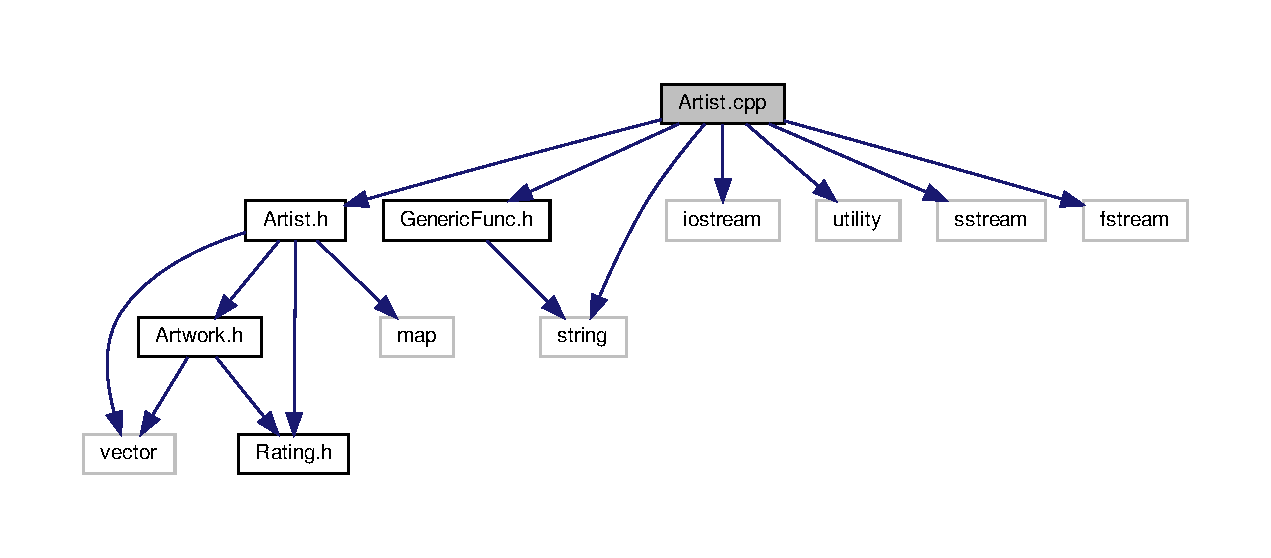
\includegraphics[width=350pt]{_artist_8cpp__incl}
\end{center}
\end{figure}

\section{Artist.\+h File Reference}
\label{_artist_8h}\index{Artist.\+h@{Artist.\+h}}
{\ttfamily \#include \char`\"{}Artwork.\+h\char`\"{}}\newline
{\ttfamily \#include \char`\"{}Rating.\+h\char`\"{}}\newline
{\ttfamily \#include $<$map$>$}\newline
{\ttfamily \#include $<$vector$>$}\newline
Include dependency graph for Artist.\+h\+:\nopagebreak
\begin{figure}[H]
\begin{center}
\leavevmode
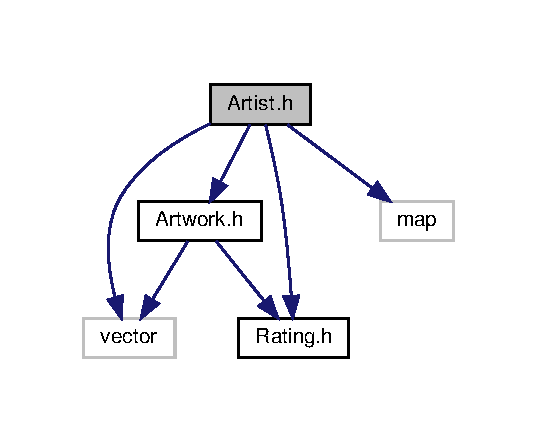
\includegraphics[width=258pt]{_artist_8h__incl}
\end{center}
\end{figure}
This graph shows which files directly or indirectly include this file\+:\nopagebreak
\begin{figure}[H]
\begin{center}
\leavevmode
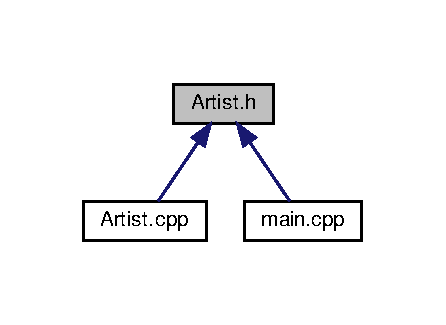
\includegraphics[width=214pt]{_artist_8h__dep__incl}
\end{center}
\end{figure}
\subsection*{Classes}
\begin{DoxyCompactItemize}
\item 
class \textbf{ Artist}
\end{DoxyCompactItemize}

\section{Artwork.\+cpp File Reference}
\label{_artwork_8cpp}\index{Artwork.\+cpp@{Artwork.\+cpp}}
{\ttfamily \#include \char`\"{}Artwork.\+h\char`\"{}}\newline
{\ttfamily \#include $<$cstddef$>$}\newline
Include dependency graph for Artwork.\+cpp\+:\nopagebreak
\begin{figure}[H]
\begin{center}
\leavevmode
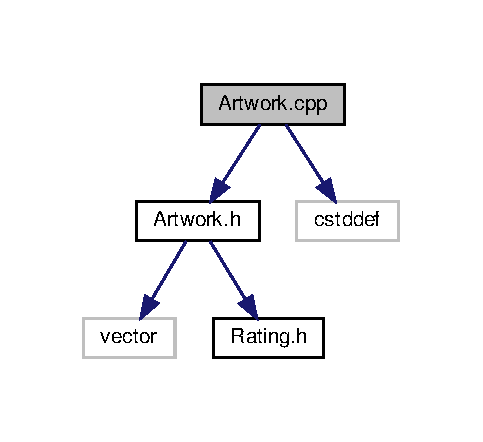
\includegraphics[width=232pt]{_artwork_8cpp__incl}
\end{center}
\end{figure}

\section{Artwork.\+h File Reference}
\label{_artwork_8h}\index{Artwork.\+h@{Artwork.\+h}}
{\ttfamily \#include $<$vector$>$}\newline
{\ttfamily \#include \char`\"{}Rating.\+h\char`\"{}}\newline
Include dependency graph for Artwork.\+h\+:\nopagebreak
\begin{figure}[H]
\begin{center}
\leavevmode
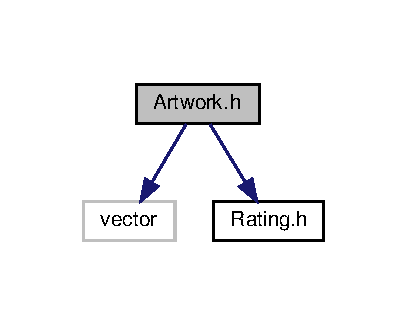
\includegraphics[width=196pt]{_artwork_8h__incl}
\end{center}
\end{figure}
This graph shows which files directly or indirectly include this file\+:\nopagebreak
\begin{figure}[H]
\begin{center}
\leavevmode
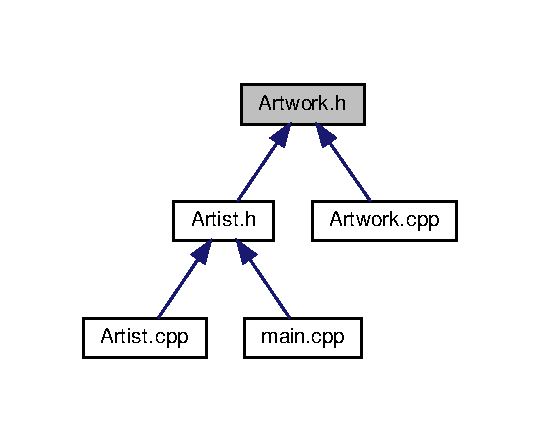
\includegraphics[width=259pt]{_artwork_8h__dep__incl}
\end{center}
\end{figure}
\subsection*{Classes}
\begin{DoxyCompactItemize}
\item 
class \textbf{ Artwork}
\end{DoxyCompactItemize}

\section{dirent.\+h File Reference}
\label{dirent_8h}\index{dirent.\+h@{dirent.\+h}}
This graph shows which files directly or indirectly include this file\+:\nopagebreak
\begin{figure}[H]
\begin{center}
\leavevmode
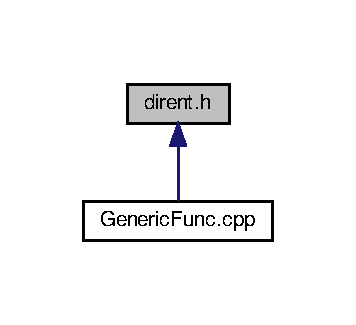
\includegraphics[width=171pt]{dirent_8h__dep__incl}
\end{center}
\end{figure}
\subsection*{Macros}
\begin{DoxyCompactItemize}
\item 
\#define \textbf{ D\+I\+R\+E\+N\+T\+\_\+\+H\+\_\+\+I\+N\+C\+L\+U\+D\+ED}
\end{DoxyCompactItemize}


\subsection{Macro Definition Documentation}
\mbox{\label{dirent_8h_a4fa796460f38104052159df94e89d209}} 
\index{dirent.\+h@{dirent.\+h}!D\+I\+R\+E\+N\+T\+\_\+\+H\+\_\+\+I\+N\+C\+L\+U\+D\+ED@{D\+I\+R\+E\+N\+T\+\_\+\+H\+\_\+\+I\+N\+C\+L\+U\+D\+ED}}
\index{D\+I\+R\+E\+N\+T\+\_\+\+H\+\_\+\+I\+N\+C\+L\+U\+D\+ED@{D\+I\+R\+E\+N\+T\+\_\+\+H\+\_\+\+I\+N\+C\+L\+U\+D\+ED}!dirent.\+h@{dirent.\+h}}
\subsubsection{D\+I\+R\+E\+N\+T\+\_\+\+H\+\_\+\+I\+N\+C\+L\+U\+D\+ED}
{\footnotesize\ttfamily \#define D\+I\+R\+E\+N\+T\+\_\+\+H\+\_\+\+I\+N\+C\+L\+U\+D\+ED}



Definition at line 83 of file dirent.\+h.


\section{Generic\+Func.\+cpp File Reference}
\label{_generic_func_8cpp}\index{Generic\+Func.\+cpp@{Generic\+Func.\+cpp}}
{\ttfamily \#include \char`\"{}Generic\+Func.\+h\char`\"{}}\newline
{\ttfamily \#include \char`\"{}dirent.\+h\char`\"{}}\newline
{\ttfamily \#include $<$unistd.\+h$>$}\newline
{\ttfamily \#include $<$limits.\+h$>$}\newline
{\ttfamily \#include $<$sstream$>$}\newline
Include dependency graph for Generic\+Func.\+cpp\+:\nopagebreak
\begin{figure}[H]
\begin{center}
\leavevmode
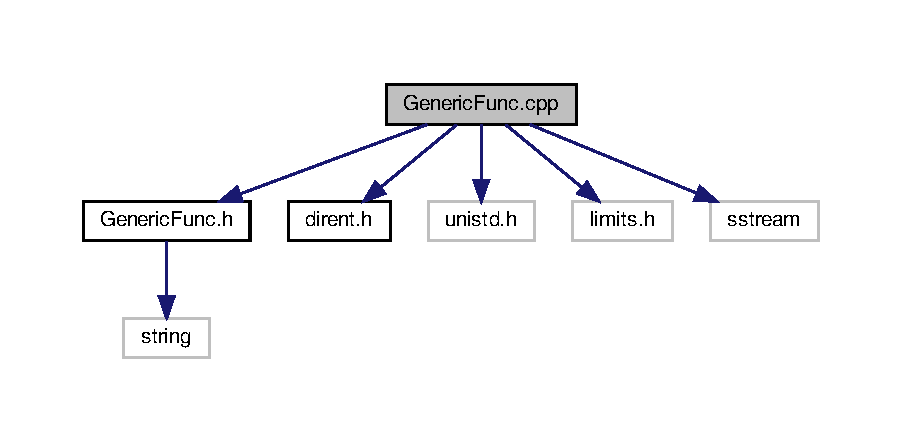
\includegraphics[width=350pt]{_generic_func_8cpp__incl}
\end{center}
\end{figure}

\section{Generic\+Func.\+h File Reference}
\label{_generic_func_8h}\index{Generic\+Func.\+h@{Generic\+Func.\+h}}
{\ttfamily \#include $<$string$>$}\newline
Include dependency graph for Generic\+Func.\+h\+:\nopagebreak
\begin{figure}[H]
\begin{center}
\leavevmode
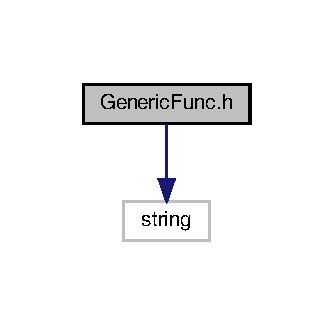
\includegraphics[width=160pt]{_generic_func_8h__incl}
\end{center}
\end{figure}
This graph shows which files directly or indirectly include this file\+:\nopagebreak
\begin{figure}[H]
\begin{center}
\leavevmode
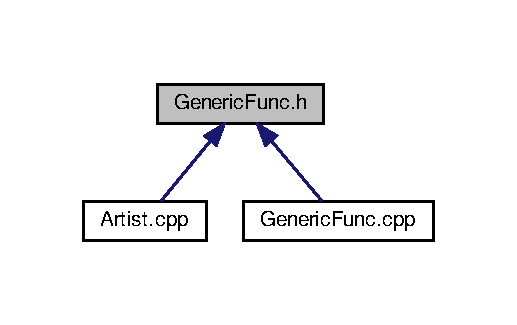
\includegraphics[width=248pt]{_generic_func_8h__dep__incl}
\end{center}
\end{figure}
\subsection*{Namespaces}
\begin{DoxyCompactItemize}
\item 
 \textbf{ gnfnc}
\end{DoxyCompactItemize}
\subsection*{Functions}
\begin{DoxyCompactItemize}
\item 
std\+::string \textbf{ gnfnc\+::get\+Executable\+Path} ()
\item 
std\+::string \textbf{ gnfnc\+::get\+Executable\+Path\+And\+Match\+It\+With\+Filename} (const std\+::string \&file\+Name)
\end{DoxyCompactItemize}

\section{main.\+cpp File Reference}
\label{main_8cpp}\index{main.\+cpp@{main.\+cpp}}
{\ttfamily \#include \char`\"{}Artist.\+h\char`\"{}}\newline
{\ttfamily \#include $<$string$>$}\newline
{\ttfamily \#include $<$iostream$>$}\newline
{\ttfamily \#include $<$fstream$>$}\newline
{\ttfamily \#include $<$sstream$>$}\newline
{\ttfamily \#include $<$map$>$}\newline
{\ttfamily \#include $<$utility$>$}\newline
{\ttfamily \#include $<$cmath$>$}\newline
{\ttfamily \#include $<$algorithm$>$}\newline
{\ttfamily \#include $<$time.\+h$>$}\newline
Include dependency graph for main.\+cpp\+:\nopagebreak
\begin{figure}[H]
\begin{center}
\leavevmode
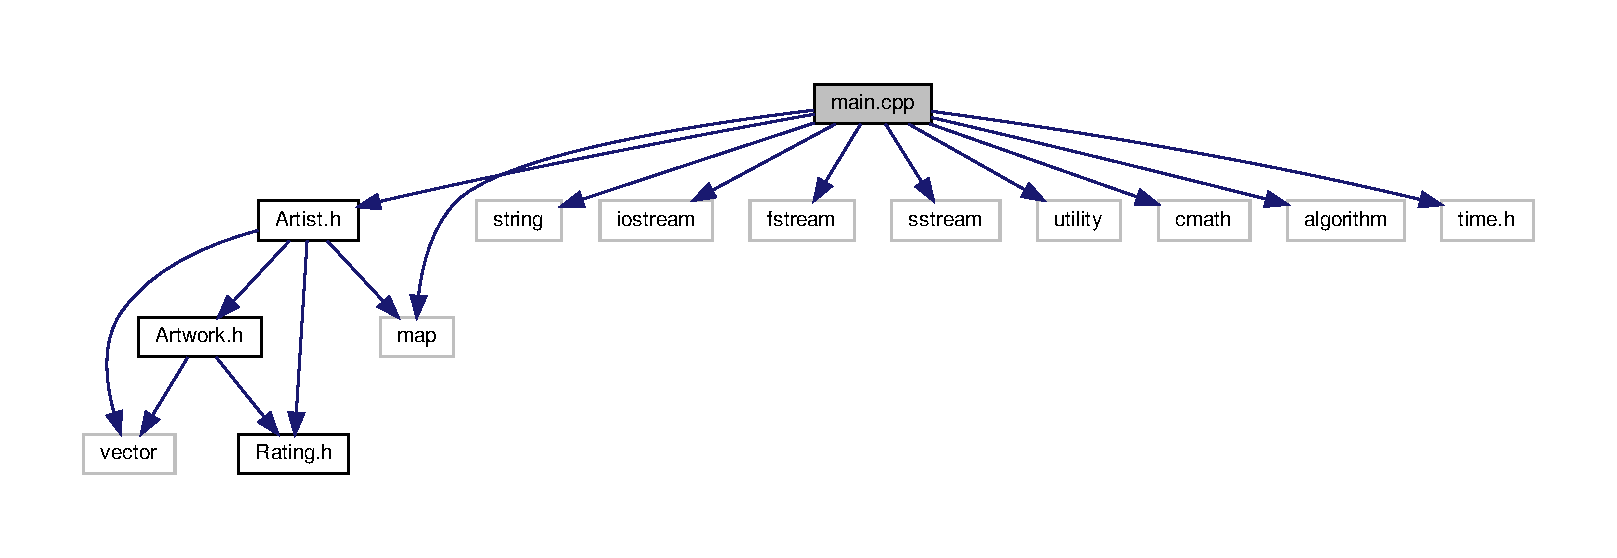
\includegraphics[width=350pt]{main_8cpp__incl}
\end{center}
\end{figure}
\subsection*{Functions}
\begin{DoxyCompactItemize}
\item 
int \textbf{ main} (int argc, char $\ast$$\ast$argv)
\end{DoxyCompactItemize}


\subsection{Function Documentation}
\mbox{\label{main_8cpp_a3c04138a5bfe5d72780bb7e82a18e627}} 
\index{main.\+cpp@{main.\+cpp}!main@{main}}
\index{main@{main}!main.\+cpp@{main.\+cpp}}
\subsubsection{main()}
{\footnotesize\ttfamily int main (\begin{DoxyParamCaption}\item[{int}]{argc,  }\item[{char $\ast$$\ast$}]{argv }\end{DoxyParamCaption})}



Definition at line 13 of file main.\+cpp.


\section{Rating.\+cpp File Reference}
\label{_rating_8cpp}\index{Rating.\+cpp@{Rating.\+cpp}}
{\ttfamily \#include \char`\"{}Rating.\+h\char`\"{}}\newline
Include dependency graph for Rating.\+cpp\+:\nopagebreak
\begin{figure}[H]
\begin{center}
\leavevmode
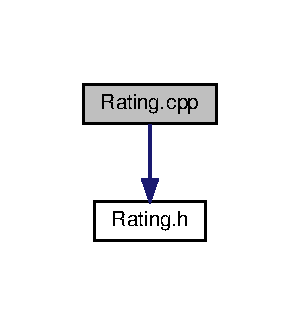
\includegraphics[width=144pt]{_rating_8cpp__incl}
\end{center}
\end{figure}

\section{Rating.\+h File Reference}
\label{_rating_8h}\index{Rating.\+h@{Rating.\+h}}
This graph shows which files directly or indirectly include this file\+:\nopagebreak
\begin{figure}[H]
\begin{center}
\leavevmode
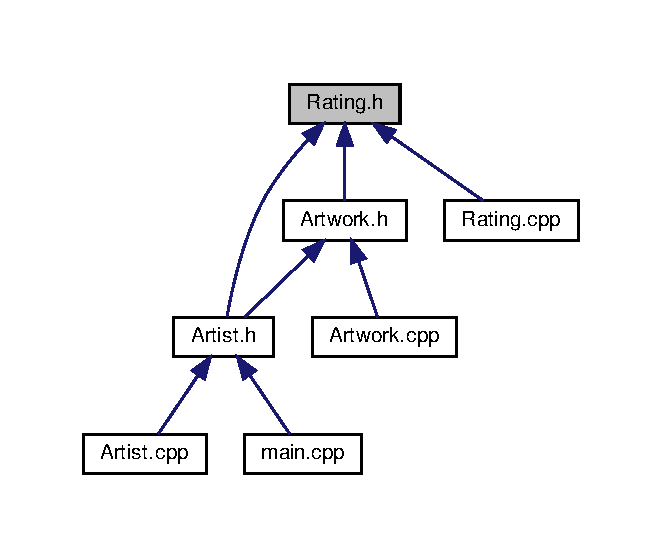
\includegraphics[width=318pt]{_rating_8h__dep__incl}
\end{center}
\end{figure}
\subsection*{Classes}
\begin{DoxyCompactItemize}
\item 
class \textbf{ Rating}
\end{DoxyCompactItemize}

%--- End generated contents ---

% Index
\backmatter
\newpage
\phantomsection
\clearemptydoublepage
\addcontentsline{toc}{chapter}{Index}
\printindex

\end{document}
